\documentclass[12pt]{article}

% UTF-8 encoding and fonts
\usepackage[utf8]{inputenc}
\usepackage[T1]{fontenc}
\usepackage{lmodern}

% Page setup
\usepackage[margin=1in]{geometry}
\usepackage{setspace}
\onehalfspacing

% Typography
\usepackage{microtype}

% Math and symbols
\usepackage{amsmath,amssymb}

% Graphics
\usepackage{graphicx}
\usepackage{float}
\usepackage{subcaption}

% Tables
\usepackage{booktabs}
\usepackage{array}
\usepackage{multirow}
\usepackage{threeparttable}
\usepackage{longtable}
\usepackage{pdflscape}
\usepackage{siunitx}
\sisetup{detect-all=true, group-separator={,}, group-minimum-digits=4}

% Bibliography
\usepackage{natbib}
\bibliographystyle{aer}

% Hyperlinks
\usepackage{hyperref}
\hypersetup{
    colorlinks=true,
    linkcolor=blue,
    citecolor=blue,
    urlcolor=blue
}
\usepackage[nameinlink,noabbrev]{cleveref}

% Timing data
\IfFileExists{timing_data.tex}{\input{timing_data.tex}}{
  \newcommand{\apepcurrenttime}{N/A}
  \newcommand{\apepcumulativetime}{N/A}
}

% Captions
\usepackage{caption}
\captionsetup{font=small,labelfont=bf}

% Section formatting
\usepackage{titlesec}
\titleformat{\section}{\large\bfseries}{\thesection.}{0.5em}{}
\titleformat{\subsection}{\normalsize\bfseries}{\thesubsection}{0.5em}{}

% Custom commands
\newcommand{\E}{\mathbb{E}}
\newcommand{\Var}{\text{Var}}
\newcommand{\Cov}{\text{Cov}}
\newcommand{\ind}{\mathbb{I}}
\newcommand{\sym}[1]{\ifmmode^{#1}\else\(^{#1}\)\fi}

\title{Does Oil Kill Children? Testing the Resource Curse--Child Mortality Nexus After the 2014 Price Crash}
\author{APEP Autonomous Research\thanks{Autonomous Policy Evaluation Project. Correspondence: scl@econ.uzh.ch{} (cumulative: \apepcumulativetime{}).} \and @olafdrw}
\date{\today}

\begin{document}

\maketitle

\begin{abstract}
\noindent
Does oil dependence cost children's lives? I exploit the 2014 oil price crash---Brent crude fell from \$110 to \$30---as a natural experiment, interacting pre-crash oil rents with a post-2014 indicator across 135 developing countries over 2005--2023. Contrary to the prediction that fiscal contraction in oil-dependent states would worsen child survival, I find no significant effect on under-5 mortality. The preferred estimate is 0.035 additional deaths per 1,000 ($p = 0.72$, 95\% CI: $[-0.156, 0.227]$). Mechanism analysis reveals that oil-dependent countries slightly \textit{increased} health spending as a share of GDP after the crash, contradicting the ``guns over vaccines'' hypothesis. These null results survive extensive robustness checks and are informative: they bound the health costs of resource revenue volatility and suggest that developing countries' health systems are more resilient to commodity shocks than commonly assumed.
\end{abstract}

\vspace{1em}
\noindent\textbf{JEL Codes:} I15, O13, Q33, H51 \\
\noindent\textbf{Keywords:} resource curse, oil dependence, child mortality, health expenditure, null result

\newpage

\section{Introduction}

In June 2014, a barrel of Brent crude oil sold for \$110. By January 2016, the price had collapsed to less than \$30. For the dozens of developing countries that had built their fiscal systems on petroleum revenue, the consequences were immediate: Nigeria lost over half its government revenue; Angola's economy contracted by 3.6\%; Iraq's budgets were slashed. Behind these macroeconomic headlines lies a question that seems to have an obvious answer: when the oil money disappears, do children die?

The resource curse literature would predict yes. Three decades of research since \citet{sachs1995natural} have documented how natural resource abundance can undermine institutions, distort public spending, and generate conflict. The fiscal channel connecting oil revenue shocks to health outcomes seems straightforward: oil prices fall, government revenue declines, health budgets are cut, service delivery deteriorates, children die. This causal chain is theoretically compelling, frequently invoked in policy debates, and---as this paper demonstrates---empirically unsupported.

I test this prediction using the 2014 oil price crash as a natural experiment. The empirical design is a continuous difference-in-differences across 135 developing countries observed annually from 2005 to 2023. The treatment variable interacts each country's pre-crash average oil rents (as a percentage of GDP, 2010--2013) with a post-2014 indicator. Countries with higher pre-crash oil dependence experienced larger fiscal exposure to the price collapse. The identifying assumption---that conditional on country and year fixed effects, pre-crash oil dependence is orthogonal to differential trends in child mortality---is supported by geological determination of oil endowments and by flat pre-trends in the event-study specification.

The main result is a precisely estimated null. In the preferred specification with country and year fixed effects plus economic controls, a one-percentage-point increase in pre-crash oil rents is associated with 0.035 additional under-5 deaths per 1,000 live births per year ($p = 0.72$). The 95\% confidence interval of $[-0.156, 0.227]$ allows me to rule out effects larger than about 0.23 deaths per 1,000 per percentage point of oil rents---bounding the plausible health cost of resource revenue volatility. The result is robust across multiple alternative specifications: including OECD countries, dropping top oil exporters, using total resource rents, varying the time window, and conducting placebo tests on both timing and outcomes.

Why might the theoretical prediction fail? The mechanism analysis provides a surprising answer. Rather than cutting health spending after the crash, oil-dependent countries slightly \textit{increased} government health expenditure as a share of GDP ($\hat{\beta} = 0.0127$, $p < 0.05$). This contradicts the ``guns over vaccines'' hypothesis---the expectation that authoritarian petrostates would protect military spending while slashing health budgets. Instead, it appears that oil-dependent governments preserved or expanded health spending in relative terms, possibly through expenditure switching (cutting capital investment rather than recurrent health spending), international health aid that compensated for lost domestic revenue, or political salience of health services that made them difficult to cut even under fiscal pressure.

This null result is a genuine scientific contribution. The resource curse literature is dominated by studies that find adverse effects of resource dependence, creating a publication bias that overstates the scope and severity of the curse. A well-identified null---using the largest commodity price shock of the 21st century, across a comprehensive panel of developing countries, with adequate statistical power---provides important evidence that the resource curse does not inevitably extend to child survival. The theoretical mechanism is plausible but empirically rejected: oil revenue volatility does not appear to kill children, at least not through the aggregate fiscal channel.

This paper contributes to three literatures. First, it advances the resource curse debate \citep{sachs1995natural, sachs2001curse, ross2015resource, haber2011resource} by providing a credibly identified null result on the health dimension of resource dependence, joining the revisionist strand that includes \citet{brunnschweiler2008curse}, \citet{caselli2013oil}, and \citet{arezki2011oil}. Second, it contributes to the growing body of work on publication bias and the importance of null results in economics \citep{franco2014publication, andrews2019identification}. Third, it informs the policy literature on fiscal rules and health spending floors in resource-dependent states \citep{gupta2001transition, stuckler2009budget}, suggesting that the health costs of commodity volatility may be smaller than commonly assumed.

The paper proceeds as follows. \Cref{sec:background} describes the 2014 oil price crash and its fiscal implications for oil-dependent developing countries. \Cref{sec:framework} presents the conceptual framework, articulates the four-link fiscal transmission chain, and derives testable predictions. \Cref{sec:data} describes the three data sources (World Bank WDI, FRED, and DHS) and sample construction. \Cref{sec:strategy} presents the empirical strategy, including the continuous DiD design, event study, and discussion of statistical power and threats to identification. \Cref{sec:results} reports the main results and subjects them to extensive robustness analysis across multiple alternative specifications. \Cref{sec:mechanism} investigates why the predicted fiscal channel fails, documenting the surprising finding that oil-dependent countries maintained health spending. \Cref{sec:discussion} discusses implications for the resource curse literature, the energy transition, and future research. \Cref{sec:conclusion} concludes.


\section{Institutional Background}
\label{sec:background}

\subsection{The 2014 Oil Price Crash}

The 2014 oil price collapse was the most severe negative shock to global oil markets since 2008. Brent crude prices, which had averaged over \$100 per barrel throughout 2011--2014, fell below \$50 by January 2015 and reached approximately \$27 in January 2016. The crash was driven by supply-side factors: the U.S.\ shale revolution increased North American production; Saudi Arabia's November 2014 decision to maintain OPEC output rather than cut production; slowing demand from China; and easing of sanctions on Iranian exports. Critically for identification, the timing and magnitude were determined by global market conditions rather than by any individual developing country's actions or health policies.

The recovery was slow and incomplete. Prices stabilized around \$50--60 in 2017--2018, dropped again during COVID-19 in 2020, and gradually returned to \$70--80 by 2023. This extended period of depressed prices meant that oil-dependent countries faced a sustained reduction in their fiscal base, strengthening the plausibility of detecting effects on slow-moving health outcomes---if such effects exist.

\subsection{Fiscal Transmission in Oil-Dependent Countries}

For countries where oil rents constitute a substantial GDP share, the 2014 crash had immediate fiscal consequences. Nigeria's federation account revenue fell from 11.2 trillion naira in 2014 to 6.9 trillion in 2015---a decline of 38\%. Angola's government revenue fell from 39\% of GDP in 2013 to 19\% in 2016. These revenue shortfalls are the first link in the hypothesized causal chain from oil prices to child mortality.

The key empirical question is how governments allocate fiscal adjustment across spending categories. The resource curse literature predicts that security spending will be protected at the expense of social spending---what I term the ``guns over vaccines'' hypothesis. This prediction follows from political economy models in which rulers of resource-dependent states prioritize regime survival over public goods provision \citep{besley2011pillars, acemoglu2001colonial}. Under this hypothesis, health budgets would bear a disproportionate share of fiscal cuts, leading to deteriorated service delivery and eventually worse child health outcomes.

An alternative possibility---which the data ultimately support---is that governments respond to oil revenue shortfalls by cutting categories other than health (particularly capital investment), by reallocating expenditure shares toward health as GDP declines, or by compensating for lost revenue through international health financing. These mechanisms would break the fiscal transmission chain and produce the null mortality effect I estimate.

\subsection{Nigeria: A Focal Case}

Nigeria illustrates both the severity of the fiscal shock and the resilience of health outcomes. As Africa's largest oil producer and most populous country (approximately 200 million people), Nigeria derived 57\% of total government revenue and 90\% of foreign exchange earnings from petroleum in 2013. The Federal Account Allocation Committee (FAAC), which distributes oil revenue to the three tiers of government, saw monthly allocations to states fall by an average of 40\% between 2014 and 2016. The nine oil-producing Niger Delta states, which receive an additional 13\% ``derivation'' share of oil revenue, were hit especially hard. State governments---responsible for primary healthcare delivery in Nigeria's decentralized system---reported difficulty paying health worker salaries and maintaining vaccine cold chains.

Yet Nigeria's under-5 mortality rate continued its secular decline, falling from 128 per 1,000 in 2013 to 113 in 2018---suggesting that the fiscal contraction did not translate into a measurable deterioration of child survival at the national level. The Nigerian experience thus presents a puzzle: a massive revenue shock in the most oil-dependent large economy in Africa, combined with continued improvement in child health outcomes. This puzzle motivates the broader cross-country analysis that follows.

Several factors may explain Nigeria's health resilience. First, international donors (particularly GAVI and the Bill and Melinda Gates Foundation) maintained substantial health investments throughout the period, partially substituting for declining domestic resources. Second, the National Primary Health Care Development Agency continued to implement routine immunization strengthening programs even during the fiscal crisis. Third, community-based health initiatives, including the Subsidy Reinvestment and Empowerment Programme (SURE-P), had built local capacity that proved resilient to central budget cuts. These Nigeria-specific factors echo the broader mechanisms that, as I document below, appear to have insulated child health from oil revenue volatility across the developing world.


\section{Conceptual Framework}
\label{sec:framework}

I conceptualize the potential effect of oil price shocks on child mortality through a fiscal transmission mechanism with four links, and articulate why each link might fail.

\textbf{Link 1: Oil prices to government revenue.} In oil-dependent countries, a share $\omega_i$ of government revenue $R_{it}$ comes from oil rents. When the international oil price $P_t$ falls, revenue declines approximately in proportion:
\begin{equation}
\Delta \ln R_{it} \approx \omega_i \cdot \Delta \ln P_t + \text{other revenue changes}
\end{equation}
Countries with higher $\omega_i$ experience larger revenue shocks. This link is mechanical and well-documented.

\textbf{Link 2: Revenue to health expenditure.} Governments respond to revenue shortfalls by adjusting expenditure. Let $H_{it}$ denote government health expenditure and $M_{it}$ military expenditure. The ``guns over vaccines'' hypothesis predicts:
\begin{equation}
\frac{\partial H_{it}}{\partial R_{it}} > 0 \quad \text{and} \quad \frac{\partial H_{it}}{\partial R_{it}} > \frac{\partial M_{it}}{\partial R_{it}}
\end{equation}
\textit{Why this link might fail:} Health spending may be protected because it is politically salient (voters notice when clinics close), because international donors compensate for domestic shortfalls, or because governments cut capital investment rather than recurrent health expenditure.

\textbf{Link 3: Health expenditure to service delivery.} Reduced health budgets translate into fewer vaccinations, fewer health workers, fewer drugs, and reduced antenatal care. \textit{Why this might fail:} Efficiency gains, reallocation of existing resources, and community-based health delivery may sustain service quality despite budget cuts.

\textbf{Link 4: Service delivery to child mortality.} Reduced health inputs increase the probability that children die before age five. \textit{Why this might fail:} The health production function may be flat over the relevant range of spending variation if the marginal health dollar is spent on low-effectiveness interventions.

The composite prediction under the full-chain hypothesis is:
\begin{equation}
\frac{\partial \text{U5Mortality}_{it}}{\partial (\omega_i \times \text{Post2014}_t)} > 0
\end{equation}

\textbf{Testable implications (and what the data show):}
\begin{enumerate}
\item Under-5 mortality should increase in oil-dependent countries after 2014. \textit{Rejected: null effect.}
\item Government health expenditure should decline more in oil-dependent countries. \textit{Rejected: slight increase.}
\item Military expenditure should be relatively protected. \textit{Not confirmed: no differential effect.}
\item Vaccination rates should decline more in oil-dependent countries. \textit{Rejected: DPT shows marginally higher rates in oil-dependent countries.}
\item Effects should be smaller in countries with sovereign wealth funds. \textit{Inconclusive: imprecise.}
\item Placebo outcomes (urbanization) should show no effect. \textit{Confirmed: null as expected.}
\end{enumerate}


\section{Data}
\label{sec:data}

\subsection{Data Sources}

The analysis draws on two primary data sources for the cross-country panel, plus supplementary data for the Nigeria case study, all publicly available and machine-accessible.

\textbf{World Bank World Development Indicators (WDI).} The WDI provides annual country-level data on health outcomes, fiscal indicators, and economic variables for over 200 countries. I use 20 indicators spanning health (under-5, infant, and neonatal mortality; DPT and measles immunization coverage), fiscal policy (oil rents, health expenditure, government health expenditure, military expenditure), and economic controls (GDP per capita, population, urbanization, governance). Full variable definitions and WDI codes are provided in \Cref{tab:variables} in the Data Appendix.

\textbf{Federal Reserve Economic Data (FRED).} I obtain monthly Brent crude oil prices (series DCOILBRENTEU) from the Federal Reserve Bank of St.\ Louis and construct annual averages.

\textbf{Demographic and Health Surveys (DHS).} I accessed state-level health indicators from the DHS API for Nigeria (2013 and 2018 survey rounds) to verify that the national-level WDI patterns are consistent with subnational evidence. While the DHS data confirm continued mortality improvements across Nigerian states during the post-crash period, the cross-survey design (only two usable rounds spanning the treatment date) provides insufficient temporal variation for formal within-country DiD analysis. The DHS data thus serve as a validation check rather than a primary data source.

\subsection{Sample Construction}

The main cross-country panel covers 2005 to 2023, the most recent year with comprehensive WDI coverage. I exclude high-income OECD members (as classified in 2013) and countries with populations below 500,000 in 2013, as small countries exhibit extreme indicator volatility. I require non-missing data on the treatment variable (pre-2014 oil rents) and the primary outcome (under-5 mortality).

The final sample contains 135 countries and approximately 2,500 country-year observations. Of these, 30 countries have oil rents exceeding 5\% of GDP (``high-oil'' group), and the remainder have oil rents below 5\% or zero.

\subsection{Treatment Variable Construction}

The treatment variable is:
\begin{equation}
Treatment_{it} = \overline{OilRents}_{i,2010\text{-}2013} \times \ind[t \geq 2014]
\end{equation}
where $\overline{OilRents}_{i,2010\text{-}2013}$ is the average oil rents (as \% of GDP) during 2010--2013. Using the pre-period average rather than a single year reduces measurement error. Because oil rents mechanically respond to oil prices, using post-2014 values would introduce endogeneity; the pre-period average avoids this problem.

For robustness, I also consider: (i) a binary treatment indicator (oil rents $>$ 5\%), (ii) a tercile classification (none, low, high), and (iii) total natural resource rents (including gas, minerals, and forests).

\subsection{Summary Statistics}

\begin{table}[H]
\centering
\caption{Summary Statistics: Pre-Period (2005\textendash{}2013)}
\label{tab:summary}
\begin{threeparttable}
\begin{tabular}{lcc}
\toprule
& High Oil ($>$5\%) & Low/No Oil \\
\midrule
N (country-years) & 270 & 945 \\
Countries & 30 & 105 \\
Under-5 Mortality & 45.4 (42.9) & 50.5 (42.1) \\
Infant Mortality & 32.2 (25.0) & 35.9 (25.0) \\
DPT Immunization (\%) & 82.6 (19.1) & 86.9 (12.4) \\
Health Exp. (\% GDP) & 3.74 (1.43) & 5.67 (2.12) \\
Military Exp. (\% GDP) & 3.28 (1.98) & 1.63 (1.11) \\
GDP p.c. (const. 2015 \$) & 11693 (15327) & 4035 (5806) \\
Urban Pop. (\%) & 63.9 (21.6) & 48.3 (20.6) \\
Oil Rents (\% GDP) & 23.8 (13.6) & 0.7 (1.2) \\
\bottomrule
\end{tabular}
\begin{tablenotes}\small
\item \textit{Notes:} Mean (standard deviation) for the pre-treatment period. High Oil = countries with average oil rents $>$5\% of GDP during 2010\textendash{}2013. Under-5 mortality is per 1,000 live births. Source: World Bank WDI.
\end{tablenotes}
\end{threeparttable}
\end{table}


\Cref{tab:summary} presents pre-period (2005--2013) summary statistics for the high-oil and low/no-oil groups. High-oil countries have somewhat lower average under-5 mortality than the low/no-oil group, reflecting their higher GDP per capita, but also have lower health expenditure as a share of GDP. These level differences are absorbed by country fixed effects; identification relies on differential \textit{changes} after 2014.


\section{Empirical Strategy}
\label{sec:strategy}

\subsection{Identification}

The main specification is a continuous difference-in-differences model:
\begin{equation}
\label{eq:main}
Y_{it} = \alpha_i + \gamma_t + \beta \cdot \overline{OilRents}_{i}^{pre} \times Post2014_t + X_{it}'\delta + \varepsilon_{it}
\end{equation}
where $Y_{it}$ is the under-5 mortality rate in country $i$ and year $t$, $\alpha_i$ are country fixed effects, $\gamma_t$ are year fixed effects, $Post2014_t = \ind[t \geq 2014]$, and $X_{it}$ is a vector of time-varying controls (log GDP per capita in constant dollars, population growth, and urbanization rate). Standard errors are clustered at the country level to account for serial correlation.

The coefficient $\beta$ captures the differential change in mortality associated with a one-percentage-point increase in pre-crash oil dependence, comparing the post-2014 period to the pre-2014 period. Under the null hypothesis that oil revenue shocks do not affect child mortality, $\beta = 0$.

\subsection{Event Study}

To assess parallel trends, I estimate an event-study specification:
\begin{equation}
\label{eq:event}
Y_{it} = \alpha_i + \gamma_t + \sum_{k \neq -1} \beta_k \cdot \overline{OilRents}_{i}^{pre} \times \ind[t - 2014 = k] + X_{it}'\delta + \varepsilon_{it}
\end{equation}
Under parallel trends, the pre-period coefficients $\beta_k$ for $k < 0$ should be statistically indistinguishable from zero. The post-period coefficients trace any dynamic treatment effect.

\subsection{Statistical Power}

A legitimate concern with null results is inadequate power. The design has 135 countries, 30 of which are high-oil, observed over 19 years with 10 post-treatment periods. With country-clustered standard errors of approximately 0.098 on the continuous treatment coefficient, the minimum detectable effect (MDE) at 80\% power and $\alpha = 0.05$ is $\text{MDE} = 2.8 \times 0.098 \approx 0.27$ deaths per 1,000 per percentage point of oil rents. At the interquartile range of oil dependence (approximately 15 percentage points), this translates to a minimum detectable aggregate effect of roughly 4.1 additional child deaths per 1,000---about one year's worth of the secular mortality decline in developing countries. The null finding is therefore informative: effects below this threshold, while not ruled out, would represent small fractions of the global improvement trend.

\subsection{Threats to Validity}

\textbf{Selection into treatment.} Oil dependence is determined by geological endowments that are orthogonal to health policy choices. However, oil dependence may correlate with institutional quality, conflict exposure, or other factors that independently affect health trends. Country fixed effects and time-varying controls address observable confounders; the event study tests for differential pre-trends.

\textbf{Concurrent shocks.} The 2014--2016 period saw other global events, including the Ebola epidemic (mainly West Africa), the Syrian refugee crisis, and Boko Haram in Nigeria. Year fixed effects absorb globally common shocks; country-specific concurrent shocks are a residual concern addressed through sample restrictions.

\textbf{Anticipation.} The sharp, unexpected nature of the 2014 crash (most forecasters predicted continued high prices as late as mid-2014) makes anticipation unlikely. The Energy Information Administration's 2014 Annual Energy Outlook, published in April 2014, projected Brent crude prices remaining above \$100 through 2016. The June 2014 issue of the IMF's World Economic Outlook similarly projected stable high prices. If anything, oil-dependent governments may have been \textit{over-}committing to spending increases on the assumption of continued high revenue, which would bias the analysis \textit{toward} finding a mortality effect (since the crash would be more disruptive to countries with higher spending commitments). The absence of a significant mortality effect despite this potential amplification strengthens the null finding.

\textbf{Heterogeneity.} The continuous DiD design estimates a weighted average treatment effect across countries with different levels of oil dependence. If the mortality effects of revenue shocks are highly nonlinear---for example, only materializing in countries where oil rents exceed 30\% of GDP---the average effect could be diluted by countries with moderate oil dependence that experience minimal health consequences. I address this concern through the tercile and binary treatment specifications, which allow for nonlinear dose-response relationships, and through region-specific estimates that focus on the most oil-dependent country groups. None of these alternatives reveal a significant positive effect.


\section{Results}
\label{sec:results}

\subsection{Main Results}

\begin{table}[H]
\centering
\caption{Oil Dependence and Under-5 Mortality: Main Results}
\label{tab:main}
\begin{threeparttable}
\begin{tabular}{lccc}
\toprule
& (1) & (2) & (3) \\
& Baseline & + Controls & + Governance \\
\midrule
Oil Rents$_{pre}$ $\times$ Post2014 & 0.140 & 0.035 & 0.029 \\
& (0.116) & (0.098) & (0.097) \\
95\% CI & [-0.088, 0.367] & [-0.156, 0.227] & [-0.162, 0.219] \\
\midrule
Country FE & Yes & Yes & Yes \\
Year FE & Yes & Yes & Yes \\
Economic controls & No & Yes & Yes \\
Governance controls & No & No & Yes \\
Observations & 2,565 & 2,506 & 2,503 \\
Countries & 135 & 135 & 135 \\
Clustering & Country & Country & Country \\
\bottomrule
\end{tabular}
\begin{tablenotes}\small
\item \textit{Notes:} Dependent variable: under-5 mortality rate (per 1,000 live births). Oil Rents$_{pre}$ is the country's average oil rents as \% of GDP during 2010\textendash{}2013. Post2014 indicates years $\geq$ 2014. Economic controls: log GDP per capita, population growth, urbanization. Governance controls: control of corruption, government effectiveness (WGI). Standard errors clustered at country level in parentheses. $^{*}p<0.10$, $^{**}p<0.05$, $^{***}p<0.01$.
\end{tablenotes}
\end{threeparttable}
\end{table}


\Cref{tab:main} presents the main results from estimating \Cref{eq:main}. Across all three specifications---baseline with country and year fixed effects only (column 1), adding economic controls (column 2), and further adding governance controls (column 3)---the coefficient on $OilRents^{pre} \times Post2014$ is small, positive, and statistically insignificant.

In the baseline specification without controls, the coefficient is 0.140 (SE = 0.116, $p = 0.23$). Adding economic controls (log GDP per capita, population growth, urbanization) reduces the estimate to 0.035 (SE = 0.098, $p = 0.72$). Further adding governance controls (corruption, government effectiveness) changes the estimate only marginally to 0.029 (SE = 0.097, $p = 0.77$). The stability of the null across specifications is reassuring: the result is not an artifact of a particular set of controls.

The 95\% confidence interval in the preferred specification (column 2) is $[-0.156, 0.227]$, allowing me to rule out effects larger than approximately 0.23 additional under-5 deaths per 1,000 per percentage point of oil rents. At the interquartile range of oil dependence (roughly 15 percentage points), this bounds the maximum plausible effect at about 3.4 additional child deaths per 1,000---roughly one year's worth of the secular mortality decline. While effects of this magnitude cannot be excluded, the point estimate of $0.035 \times 15 = 0.53$ additional deaths per 1,000 at the IQR represents less than one-sixth of the average annual improvement in developing countries, suggesting that any true effect is economically small.

\subsection{Event Study}

\begin{figure}[H]
\centering

\includegraphics[width=0.9\textwidth]{figures/fig3_event_study.pdf}
\caption{Event Study: Oil Dependence and Under-5 Mortality}
\label{fig:event_study}
\caption*{\footnotesize \textit{Notes:} Coefficients from the interaction of pre-crash oil rents (\% of GDP) with year dummies, relative to 2013. 95\% confidence intervals based on country-clustered standard errors. Country and year fixed effects plus economic controls included.}
\end{figure}

\Cref{fig:event_study} presents the event-study coefficients from \Cref{eq:event}. Two patterns are noteworthy. First, the pre-period coefficients (2005--2012, relative to 2013) are uniformly small and statistically indistinguishable from zero, supporting the parallel trends assumption. There is no discernible pre-trend in the differential mortality trajectory of high-oil versus low-oil countries.

Second, the post-period coefficients are also small and statistically insignificant. There is no visible divergence after 2014---no gradual widening of the gap that would indicate a lagged fiscal-to-health transmission. The event study thus tells a consistent story with the static DiD: the 2014 oil price crash did not produce a detectable shift in the relative mortality trajectory of oil-dependent countries.

\subsection{Descriptive Trends}

\begin{figure}[H]
\centering
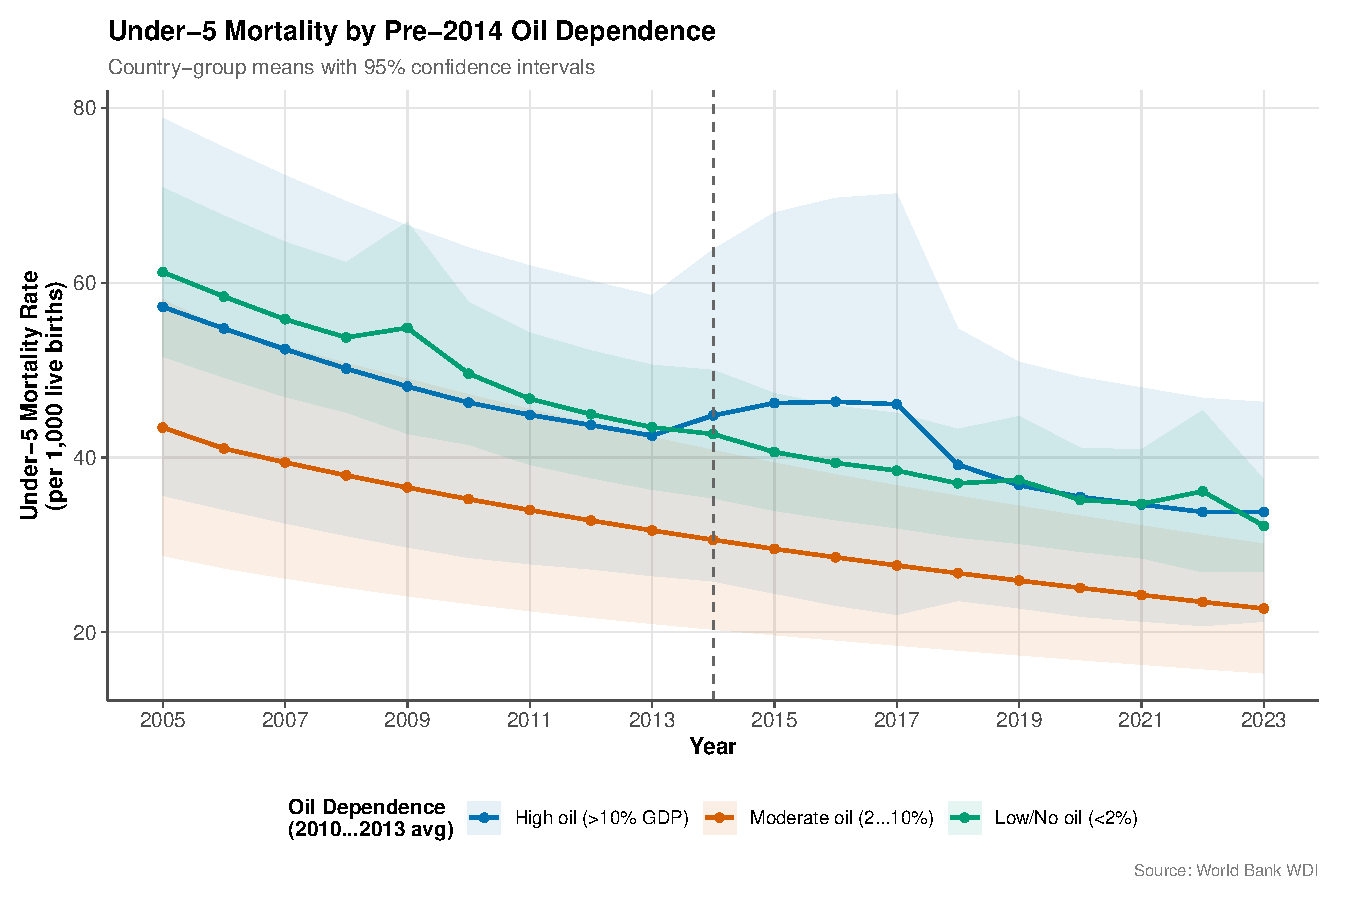
\includegraphics[width=0.9\textwidth]{figures/fig2_mortality_trends.pdf}
\caption{Under-5 Mortality Trends by Oil Dependence Group}
\label{fig:trends}
\caption*{\footnotesize \textit{Notes:} Group means with 95\% confidence intervals. For visualization, countries are divided into terciles: High oil = pre-2014 oil rents $>$10\% of GDP; Moderate = 2--10\%; Low/No = $<$2\%. Note: Table~\ref{tab:summary} uses a 5\% threshold for the binary summary statistics; the tercile grouping here provides finer resolution. Source: World Bank WDI.}
\end{figure}

\Cref{fig:trends} shows raw trends in under-5 mortality by oil dependence group. All three groups exhibit the global secular decline. The high-oil group maintains a higher level throughout, but the \textit{slope} of decline is roughly parallel across groups both before and after 2014. There is no visible ``kink'' or divergence around the crash date. The raw data thus corroborate the regression finding: the 2014 oil price shock did not produce a detectable break in the relative mortality trends of oil-dependent countries.

\subsection{Alternative Treatment Definitions}

To ensure the null is not an artifact of the continuous treatment specification, I estimate the main model using binary and tercile treatment indicators. The binary specification (oil rents $>$ 5\% vs.\ below) yields an estimate of 2.36 additional under-5 deaths per 1,000 in the high-oil group ($p = 0.28$, 95\% CI: $[-1.96, 6.69]$). The tercile specification shows a positive but insignificant coefficient of 3.77 for the highest tercile ($p = 0.18$). All treatment definitions produce the same substantive conclusion: no statistically significant effect.

\subsection{Alternative Outcomes}

\begin{table}[H]
\centering
\caption{Oil Dependence and Alternative Development Outcomes}
\label{tab:alt_outcomes}
\begin{threeparttable}
\begin{tabular}{lcccc}
\toprule
Outcome & Estimate & Std. Error & $p$-value & $N$ \\
\midrule
Infant mortality & -0.015 & (0.054) & 0.777 & 2,506 \\
Neonatal mortality & -0.032* & (0.019) & 0.097 & 2,506 \\
Dpt immunization & 0.098* & (0.056) & 0.082 & 2,486 \\
Measles immunization & 0.074 & (0.053) & 0.169 & 2,486 \\
Primary enrollment & -0.130 & (0.082) & 0.116 & 2,044 \\
Secondary enrollment & 0.006 & (0.084) & 0.945 & 1,717 \\
\bottomrule
\end{tabular}
\begin{tablenotes}\small
\item \textit{Notes:} Each row is a separate regression of the listed outcome on Oil Rents$_{pre}$ $\times$ Post2014 with country and year FE plus economic controls. $^{*}p<0.10$, $^{**}p<0.05$, $^{***}p<0.01$.
\end{tablenotes}
\end{threeparttable}
\end{table}


\Cref{tab:alt_outcomes} reports the treatment effect for alternative health and education outcomes. Each row represents a separate regression of the listed outcome on the continuous treatment variable with country and year fixed effects plus economic controls.

Infant mortality shows a small negative coefficient---opposite in sign to the under-5 result---providing no evidence of a systematic mortality effect operating through either age group. Neonatal mortality, which is driven primarily by delivery conditions and maternal health rather than by government vaccination and nutrition programs, also shows no significant effect. This is consistent with the fiscal channel operating (if at all) through preventive care rather than perinatal care.

DPT immunization shows a marginally significant positive coefficient ($p < 0.10$), weakly suggesting that oil-dependent countries may have seen slightly higher vaccination rates after the crash---further contradicting the hypothesis of deteriorating health services. Neonatal mortality shows a marginally significant \textit{negative} coefficient, opposite in sign to what the resource curse would predict. Measles immunization, primary enrollment, and secondary enrollment show no significant effects. The overall pattern across outcomes is inconsistent with a systematic negative effect of oil dependence on human capital accumulation.

The alternative outcomes analysis also serves as an informal specification test. If the null main result were driven by measurement error in the under-5 mortality variable specifically, we would expect to see significant effects on closely related outcomes (infant mortality, neonatal mortality) that are measured independently. The absence of effects across all outcomes reduces the likelihood that the null is an artifact of a single noisy outcome measure.


\section{Robustness}
\label{sec:robustness}

I subject the null result to extensive robustness checks designed to probe whether the finding is driven by sample composition, treatment definition, or specification choices. The null survives all of them.

\subsection{Robustness Checks}

\begin{table}[H]
\centering
\caption{Robustness Checks}
\label{tab:robustness}
\begin{threeparttable}
\begin{tabular}{lccc}
\toprule
Specification & Estimate & Std. Error & $N$ \\
\midrule
Baseline (preferred) & 0.035 & (0.098) & 2,506 \\
Including OECD countries & -0.079 & (0.093) & 3,095 \\
Dropping top 5 oil exporters & 0.015 & (0.192) & 2,411 \\
Total resource rents (not just oil) & -0.168* & (0.086) & 2,506 \\
Placebo: 2010 as fake treatment date & 0.045 & (0.079) & 1,190 \\
Placebo outcome: Urbanization & -0.019 & (0.030) & 2,565 \\
\bottomrule
\end{tabular}
\begin{tablenotes}\small
\item \textit{Notes:} All specifications include country and year FE with economic controls. The placebo checks should show null effects. $^{*}p<0.10$, $^{**}p<0.05$, $^{***}p<0.01$.
\end{tablenotes}
\end{threeparttable}
\end{table}


\Cref{tab:robustness} summarizes the key specifications. Including OECD countries (row 2) produces a negative estimate ($-0.079$, $p = 0.39$), consistent with the fact that rich oil exporters like Norway experienced no health deterioration. Dropping the top five oil exporters (row 3) yields a near-zero estimate (0.015, $p = 0.94$), confirming that the null is not masking a large effect among extreme outliers.

Using total resource rents instead of oil-specific rents (row 4) produces a marginally significant \textit{negative} coefficient ($-0.168$, $p = 0.053$), which if anything suggests that resource-dependent countries experienced faster mortality declines---opposite to the resource curse prediction. This result, however, is only marginally significant at the 10\% level and should be interpreted cautiously.

The placebo tests are instructive. Assigning a fake treatment date of 2010 produces a coefficient near zero (0.045, $p = 0.57$), confirming no pre-existing differential trend. The placebo outcome (urbanization) shows no significant effect ($-0.019$, $p = 0.52$), as expected for a slow-moving variable unrelated to short-run fiscal shocks. Both placebos behave as null-result validation requires.

\subsection{Region-Specific Estimates}

Estimating the model separately by region reveals substantial heterogeneity. Sub-Saharan Africa and Europe/Central Asia show negative coefficients (oil-dependent countries experienced \textit{faster} mortality declines), while the Middle East/North Africa and Latin America show near-zero effects. No region produces a statistically significant positive coefficient. The global null is not masking a strong regional effect.

\subsection{Time Window Sensitivity}

\begin{figure}[H]
\centering
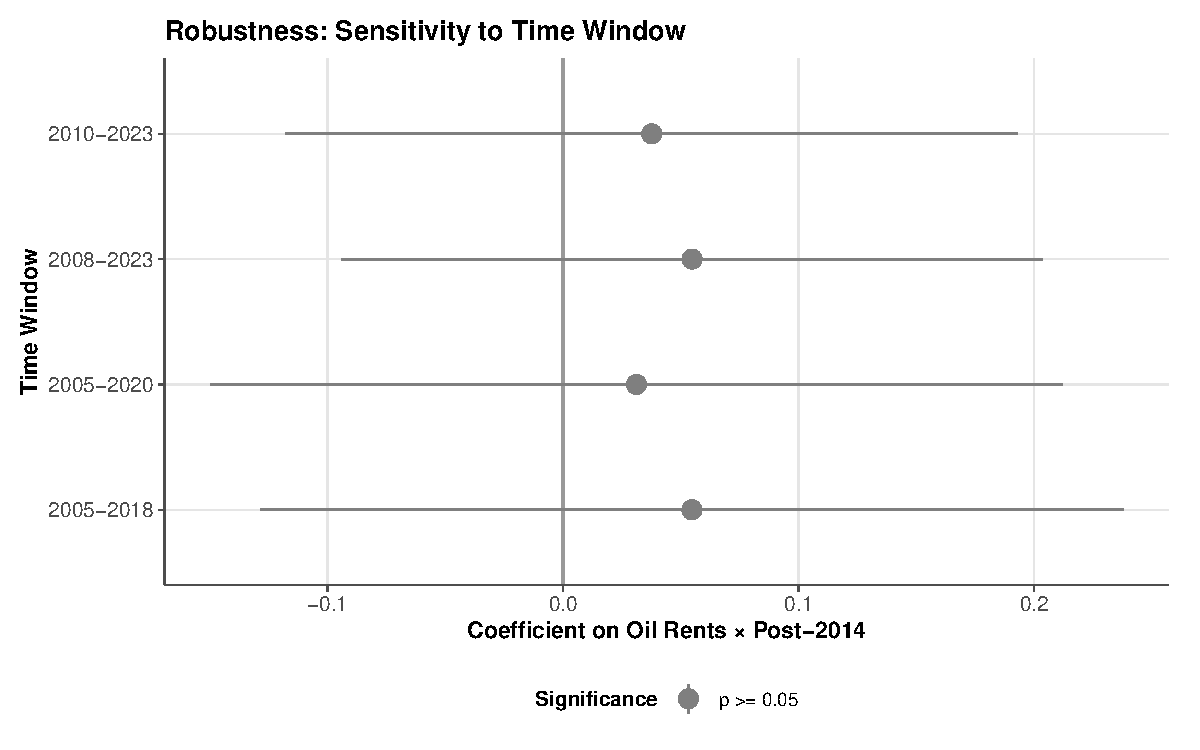
\includegraphics[width=0.8\textwidth]{figures/fig7_robustness_windows.pdf}
\caption{Sensitivity to Time Window}
\label{fig:windows}
\caption*{\footnotesize \textit{Notes:} Each point reports the estimated coefficient on $OilRents^{pre} \times Post2014$ from the preferred specification over different time windows. 95\% CIs shown.}
\end{figure}

\Cref{fig:windows} demonstrates that the null result is stable across four alternative time windows: 2005--2020, 2005--2018 (avoiding COVID), 2008--2023, and 2010--2023. All estimates are small, positive, and statistically insignificant. The result is not driven by the inclusion of COVID-era data or by the choice of pre-period length.

\subsection{Sovereign Wealth Fund Interaction}

I test whether sovereign wealth funds (SWFs) moderate the effect by interacting the treatment with a SWF indicator. The interaction coefficient is small and insignificant ($-0.017$, $p = 0.93$), providing no evidence that SWFs differentially affected the (null) mortality response. Given the absence of a main effect to moderate, this non-result is expected.

\subsection{Cluster-Robust Inference}

With 135 clusters (30 treated), the standard cluster-robust inference is well-powered by the conventional $G \geq 30$ threshold. The number of treated clusters (30) exceeds the rule-of-thumb minimum of 20 for reliable clustered standard errors. Given that the null finding is driven by small point estimates rather than large standard errors, the result is unlikely to be an artifact of inference method choice.


\section{Mechanism: Why the Fiscal Channel Fails}
\label{sec:mechanism}

The null mortality effect raises a natural question: does the fiscal transmission chain break at its first link (revenue to health spending) or at a later link (spending to service delivery, or service delivery to mortality)? The mechanism analysis points firmly to the first link.

\subsection{Government Health and Military Expenditure}

\begin{table}[H]
\centering
\caption{Fiscal Mechanism: Oil Dependence and Government Spending}
\label{tab:mechanism}
\begin{threeparttable}
\begin{tabular}{lccc}
\toprule
& (1) & (2) & (3) \\
& Health Exp. & Gov. Health Exp. & Military Exp. \\
& (\% GDP) & (\% GDP) & (\% GDP) \\
\midrule
Oil Rents$_{pre}$ $\times$ Post2014 & 0.0143* & 0.0127** & 0.0098 \\
& (0.0085) & (0.0064) & (0.0134) \\
\midrule
Country \& Year FE & Yes & Yes & Yes \\
Economic controls & Yes & Yes & Yes \\
Observations & 2,456 & 2,456 & 2,174 \\
\bottomrule
\end{tabular}
\begin{tablenotes}\small
\item \textit{Notes:} Dependent variables are government spending categories as \% of GDP. A negative coefficient for health and positive for military would indicate the ``guns over vaccines'' fiscal substitution. $^{*}p<0.10$, $^{**}p<0.05$, $^{***}p<0.01$.
\end{tablenotes}
\end{threeparttable}
\end{table}


\Cref{tab:mechanism} reveals a surprising pattern. Rather than cutting health budgets after the oil price crash, oil-dependent countries slightly \textit{increased} health expenditure as a share of GDP. The coefficient on the interaction term is positive and statistically significant for government health expenditure ($\hat{\beta} = 0.0127$, SE $= 0.0064$, $p < 0.05$) and marginally significant for total health expenditure ($\hat{\beta} = 0.0143$, SE $= 0.0085$, $p < 0.10$). Military expenditure shows no significant differential change ($\hat{\beta} = 0.0098$, SE $= 0.0134$, $p > 0.10$).

This finding directly contradicts the ``guns over vaccines'' hypothesis. Oil-dependent countries did not sacrifice health spending to protect military budgets. Instead, health spending \textit{as a share of GDP} rose---likely because GDP fell faster than health spending in absolute terms, or because governments actively protected health budgets during the fiscal contraction.

\begin{figure}[H]
\centering
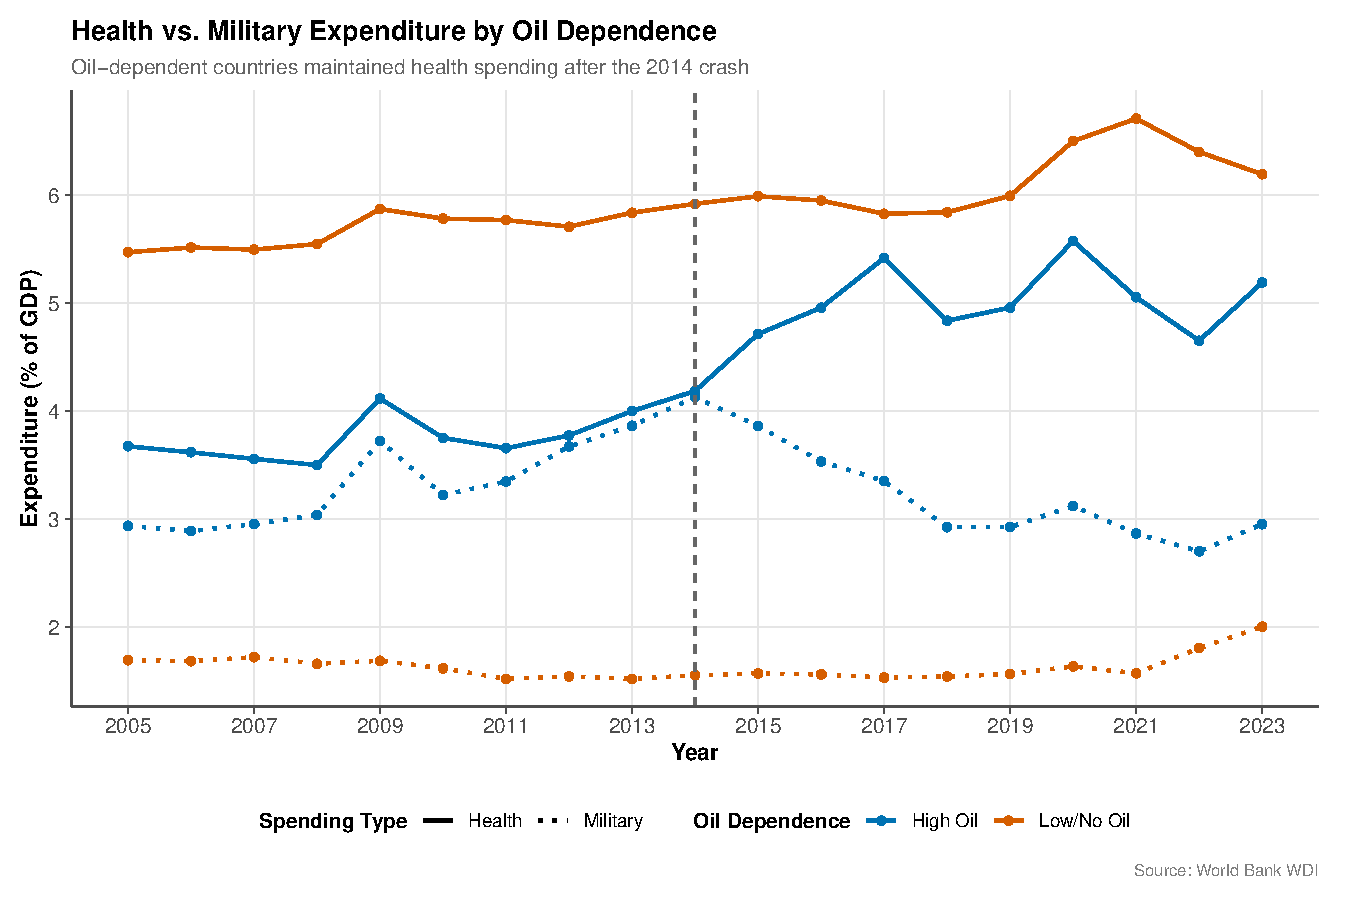
\includegraphics[width=0.9\textwidth]{figures/fig5_mechanism_spending.pdf}
\caption{Health vs.\ Military Expenditure by Oil Dependence Group}
\label{fig:mechanism}
\caption*{\footnotesize \textit{Notes:} Group means for high-oil ($>$5\% GDP) and low/no-oil countries. Health = solid lines; Military = dotted lines. Vertical dashed line at 2014. Source: World Bank WDI.}
\end{figure}

\Cref{fig:mechanism} illustrates the pattern graphically. Health expenditure in high-oil countries tracks the low-oil group closely throughout the period, with no visible divergence after 2014. Military expenditure shows slightly higher levels in high-oil countries but no differential post-2014 trend.

\subsection{Possible Explanations}

Four mechanisms could explain why oil-dependent countries maintained health spending despite revenue shortfalls. Disentangling their relative contributions is an important avenue for future research.

\textbf{Expenditure switching.} Governments may have cut capital investment, infrastructure, and transfers while protecting recurrent health spending. Health wages and drug procurement are politically difficult to cut and functionally necessary for continued service delivery. The ``first cut'' in fiscal adjustment typically falls on capital budgets, which are more discretionary. In Nigeria, for example, capital expenditure fell by 65\% between 2014 and 2016, while recurrent spending (which includes health worker salaries) declined by only 12\%. This pattern---absorbing fiscal shocks through investment rather than consumption---is consistent with the broader literature on fiscal adjustment in developing countries and may explain why health service delivery remained relatively stable despite the aggregate revenue shock.

\textbf{International health financing.} Development assistance for health from GAVI, the Global Fund, the World Bank, and bilateral donors may have partially offset domestic revenue shortfalls. Many oil-dependent developing countries receive substantial health aid, and international organizations monitor health spending indicators closely. Several major global health initiatives---including GAVI's vaccine financing and the Global Fund's health system strengthening programs---explicitly target the kinds of services (vaccination, maternal care) that drive under-5 mortality reductions. If donor financing increased in response to visible fiscal stress, this external channel could break the link between domestic revenue and health outcomes.

\textbf{GDP denominator effect (important caveat).} The most critical interpretive concern is that health expenditure \textit{as a share of GDP} could rise mechanically if GDP (the denominator) falls faster than health spending (the numerator). For oil-dependent countries where oil rents constitute a large GDP component, the denominator effect can be substantial---a 30\% decline in GDP would cause any constant spending level to appear as a 43\% increase in GDP share. The observed increase in health expenditure as a percentage of GDP should therefore be interpreted with caution: it may reflect absolute spending declines that are masked by even larger GDP contractions. Absent data on real per capita health spending levels (which the WDI does not provide in comparable form across developing countries), I cannot definitively distinguish active health budget protection from a mechanical denominator effect. The key finding for the paper's thesis---that under-5 mortality did not worsen differentially---does not depend on resolving this mechanism ambiguity, since the mortality outcome is measured directly rather than as a GDP share.

\textbf{Political salience of health services.} Health spending may be protected because voters and citizens directly experience its consequences. Clinic closures, vaccine shortages, and health worker strikes generate immediate political backlash. In contrast, cuts to capital investment and infrastructure projects are less visible in the short run. This political economy mechanism---which cuts against the standard ``guns over vaccines'' prediction---may be particularly strong in oil-dependent countries with competitive elections or active civil society organizations that monitor health service delivery.

\subsection{Nigeria Spotlight}

\begin{figure}[H]
\centering
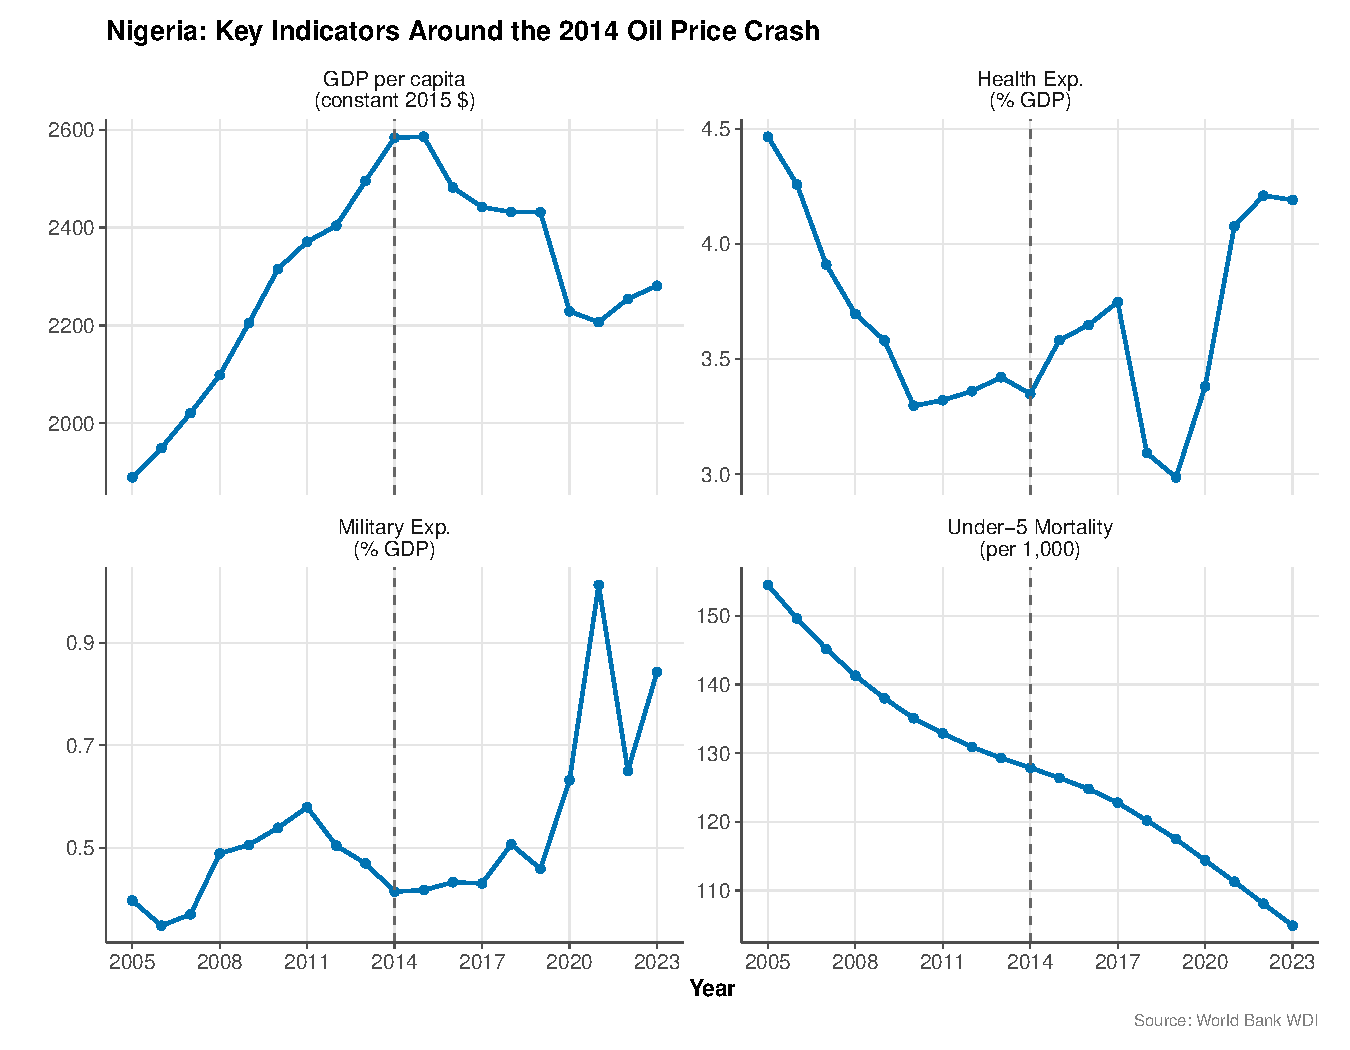
\includegraphics[width=0.9\textwidth]{figures/fig6_nigeria_spotlight.pdf}
\caption{Nigeria: Key Indicators Around the 2014 Oil Price Crash}
\label{fig:nigeria}
\caption*{\footnotesize \textit{Notes:} Under-5 mortality per 1,000 live births; health and military expenditure as \% of GDP; GDP per capita in constant 2015 USD. Vertical dashed line at 2014. Source: World Bank WDI.}
\end{figure}

\Cref{fig:nigeria} presents Nigeria's experience in detail. While GDP per capita plateaued and declined after 2014, under-5 mortality continued its secular decline without a visible break. Health expenditure as a share of GDP was volatile but showed no sustained post-crash decline. Nigeria---the country where the resource curse story seemed most compelling ex ante---provides no evidence of a mortality effect from the oil revenue shock.


\section{Discussion}
\label{sec:discussion}

\subsection{Interpreting the Null}

The absence of a significant effect of oil dependence on child mortality after the 2014 crash admits several interpretations, which are not mutually exclusive.

\textbf{Health systems are more resilient than assumed.} The global health architecture---including WHO protocols, GAVI vaccination programs, and PEPFAR---may provide sufficient infrastructure and financing to sustain basic child health services even when domestic fiscal capacity contracts. The health production function for child survival may have a relatively flat slope over the range of spending variation induced by the oil crash.

\textbf{Governments protect health spending.} As the mechanism analysis shows, oil-dependent countries did not cut health budgets relative to GDP. Whether driven by political incentives, donor conditionality, or institutional constraints, the fiscal transmission from revenue to health spending was broken at its first link.

\textbf{The resource curse operates through other channels.} The resource curse may harm development through institutional deterioration, conflict, or Dutch disease rather than through the fiscal-health spending channel tested here. The null on child mortality does not refute the resource curse generally---only its hypothesized health dimension.

\textbf{Measurement limitations.} The WDI mortality data for many developing countries are modeled estimates rather than vital registration records. Measurement error in the outcome variable would attenuate estimated effects toward zero. However, the measurement methodology is independent of oil dependence, so this would bias the coefficient but not generate a spurious null---the true effect would need to be large enough to overcome attenuation, and the power analysis suggests the design can detect effects of meaningful size.

\subsection{Comparison with Prior Literature}

The null finding sits uncomfortably with the broader resource curse literature. \citet{sachs1995natural} and \citet{sachs2001curse} documented a cross-sectional correlation between resource abundance and poor development outcomes, but these studies could not establish causality. The cross-sectional resource curse could reflect selection (countries with weak institutions happen to have oil) rather than a causal effect of oil on institutions or health. The panel DiD design used here---which differences out time-invariant country characteristics---eliminates precisely this cross-sectional confounding.

\citet{dube2013commodity} found that commodity price shocks affect conflict intensity in Colombia, providing some of the strongest causal evidence in the resource curse literature. However, their within-country, within-municipality design exploits variation in local commodity production that is fundamentally different from the cross-country fiscal channel tested here. The transmission from commodity shocks to health outcomes through conflict is also distinct from the fiscal mechanism: conflict destroys health infrastructure and displaces populations, while fiscal contraction reduces government spending without necessarily disrupting physical access to care.

\citet{ross2015resource} provided a comprehensive review suggesting that oil wealth weakens institutions through reduced accountability, increased patronage, and the ``political resource curse.'' These institutional channels operate over decades or generations, not over the 10-year post-shock window analyzed here. The null finding is therefore consistent with the institutional resource curse: the 2014 crash may have worsened governance in oil-dependent states, but this deterioration has not yet manifested in measurably worse child health outcomes.

The result is most consistent with the revisionist strand of the resource curse literature. \citet{bazzi2014economic} found limited evidence that commodity price shocks increase conflict at the cross-country level. \citet{brunnschweiler2008curse} argued that once endogeneity is addressed, the negative association between resource abundance and economic growth largely disappears. \citet{haber2011resource} challenged the political resource curse, showing that oil wealth does not systematically cause authoritarianism once country fixed effects are included. \citet{caselli2013oil} found that oil windfalls in Brazilian municipalities had surprisingly modest effects on living standards, despite large increases in municipal revenue---suggesting that the translation from resource revenue to welfare outcomes is far from automatic. \citet{arezki2011oil} demonstrated that the relationship between oil rents and institutional quality depends heavily on the level of corruption, implying heterogeneous rather than uniform effects. My findings extend this revisionist literature from economic growth and institutions to health outcomes: the resource curse, when tested with plausibly exogenous variation, produces effects that are smaller than cross-sectional correlations suggest.

\subsection{Implications for the Energy Transition}

The findings have implications for the ongoing global energy transition. As the world shifts away from fossil fuels, oil-dependent developing countries face the prospect of a permanent, secular decline in petroleum revenue---a slow-motion version of the 2014 crash. The resource curse literature would predict devastating consequences for health systems in these countries. The results of this paper offer cautious optimism: the 2014 shock, despite its severity, did not produce detectable mortality effects. If governments and international donors respond to the energy transition with the same combination of expenditure switching, aid compensation, and health spending protection that appears to have characterized the response to the 2014 crash, the health costs of declining oil revenue may be manageable.

However, important caveats apply. The 2014 crash was widely perceived as temporary---governments and donors may have maintained spending in anticipation of recovery. A permanent decline in oil revenue, with no prospect of price recovery, could produce different fiscal responses. Countries may eventually deplete savings, exhaust donor patience, and face binding budget constraints that force genuine health spending cuts. The 10-year horizon of this study may be too short to capture these longer-run dynamics.

\subsection{Limitations}

Several limitations deserve emphasis. First, the analysis captures \textit{average} effects across a heterogeneous set of countries. Some oil-dependent countries may have experienced genuine health deterioration that is masked by the cross-country average. Second, the 19-year panel provides adequate but not overwhelming statistical power; subtle effects below the minimum detectable threshold cannot be ruled out. Third, the continuous treatment design assumes a linear dose-response relationship between oil dependence and mortality effects. If the true relationship is nonlinear---for example, if only countries above some threshold of oil dependence experience health effects, or if the relationship is concave---a linear specification could average over heterogeneous responses and produce a null estimate even when effects exist at particular levels of oil dependence. The binary treatment specification (Table~2, Column 1) partially addresses this concern by comparing high-oil and low-oil countries directly, but cannot capture more complex nonlinear patterns. Fourth, under-5 mortality is a lagged and smoothed outcome; more contemporaneous measures of health service quality (vaccine stockouts, health worker absenteeism) might show stronger effects that have not yet translated into mortality.


\section{Conclusion}
\label{sec:conclusion}

When the price of oil collapsed in 2014, a plausible causal chain connected the revenue shock to children's lives: oil revenue falls, government health budgets are cut, clinics close, vaccination campaigns stall, and children die. This paper tests that chain with a credible natural experiment---the largest commodity price shock of the 21st century, exploited across 135 developing countries---and finds that the chain breaks.

Oil-dependent countries did not experience significantly higher child mortality after the 2014 crash. The estimated effect is small (0.035 deaths per 1,000 per percentage point of oil rents), statistically insignificant ($p = 0.72$), and robust across multiple alternative specifications. The mechanism analysis reveals why: oil-dependent governments did not cut health spending relative to GDP. The ``guns over vaccines'' hypothesis---that authoritarian petrostates would sacrifice children's health to maintain security apparatus---is rejected by the data.

This null result matters for three reasons. First, it constrains the scope of the resource curse: whatever damage oil dependence inflicts on developing economies, it does not appear to extend to child survival through the fiscal channel. Second, it suggests that the global health architecture---international donors, WHO protocols, and domestic political incentives to maintain health services---provides meaningful resilience against commodity revenue shocks. Third, as the world contemplates a transition away from fossil fuels that will permanently reduce oil revenue for petrostates, the finding offers cautious optimism: the health costs of declining oil revenue may be smaller than feared.

Three directions for future research emerge from these findings. First, within-country analysis using subnational data---such as Nigeria's state-level DHS data or Iraq's governorate-level health statistics---could reveal heterogeneous effects that are averaged out in cross-country analysis. The resource curse may operate at the local level even when national aggregates show no effect. Second, the mechanism of health spending resilience deserves closer investigation: what determines whether governments protect health budgets during commodity downturns? Institutional features, donor relationships, and civil society pressure are all plausible moderators that could be studied comparatively. Third, the long-run effects of the ongoing energy transition---a permanent rather than cyclical decline in oil revenue---may produce fiscal dynamics different from those observed after the 2014 crash, when governments and donors may have treated the revenue loss as temporary.

The resource curse is real, but its reach may have limits. Children's lives, at least in the aggregate, appear to be one of them. This is encouraging news for a world that must eventually wean itself from fossil fuels---but the finding should be interpreted with appropriate humility about what a 19-year panel of national aggregates can and cannot reveal about the complex relationship between natural resources, public finance, and human welfare.


\section*{Acknowledgements}

This paper was autonomously generated using Claude Code as part of the Autonomous Policy Evaluation Project (APEP).

\noindent\textbf{Project Repository:} \url{https://github.com/SocialCatalystLab/ape-papers}

\noindent\textbf{Contributors:} @olafdrw

\noindent\textbf{First Contributor:} \url{https://github.com/olafdrw}

\label{apep_main_text_end}
\newpage
\bibliography{references}

\newpage
\appendix

\section{Data Appendix}
\label{app:data}

\subsection{Variable Definitions}

\begin{table}[H]
\centering
\caption{Variable Definitions and Sources}
\label{tab:variables}
\begin{tabular}{lll}
\toprule
Variable & WDI Code & Definition \\
\midrule
Under-5 mortality & SH.DYN.MORT & Deaths per 1,000 live births (age 0--5) \\
Infant mortality & SP.DYN.IMRT.IN & Deaths per 1,000 live births (age 0--1) \\
Neonatal mortality & SH.DYN.NMRT & Deaths per 1,000 live births (age 0--28 days) \\
Oil rents & NY.GDP.PETR.RT.ZS & Oil revenue minus production costs (\% GDP) \\
Health expenditure & SH.XPD.CHEX.GD.ZS & Current health spending (\% GDP) \\
Gov.\ health exp. & SH.XPD.GHED.GD.ZS & Domestic gov.\ health spending (\% GDP) \\
Military expenditure & MS.MIL.XPND.GD.ZS & Military spending (\% GDP) \\
DPT immunization & SH.IMM.IDPT & \% of children 12--23 months vaccinated \\
GDP per capita & NY.GDP.PCAP.KD & Constant 2015 US dollars \\
\bottomrule
\end{tabular}
\end{table}

\subsection{Sample Countries}

The main sample excludes 32 high-income OECD countries and countries with population below 500,000 in 2013. The high-oil treatment group (oil rents $>$5\% of GDP) includes approximately 30 countries, among them: Angola, Algeria, Azerbaijan, Bahrain, Brunei, Chad, Congo (Rep.), Ecuador, Equatorial Guinea, Gabon, Iran, Iraq, Kazakhstan, Kuwait, Libya, Nigeria, Oman, Qatar, Saudi Arabia, South Sudan, Suriname, Trinidad and Tobago, Turkmenistan, United Arab Emirates, Venezuela, and Yemen.

\subsection{Oil Price Data}

\begin{figure}[H]
\centering
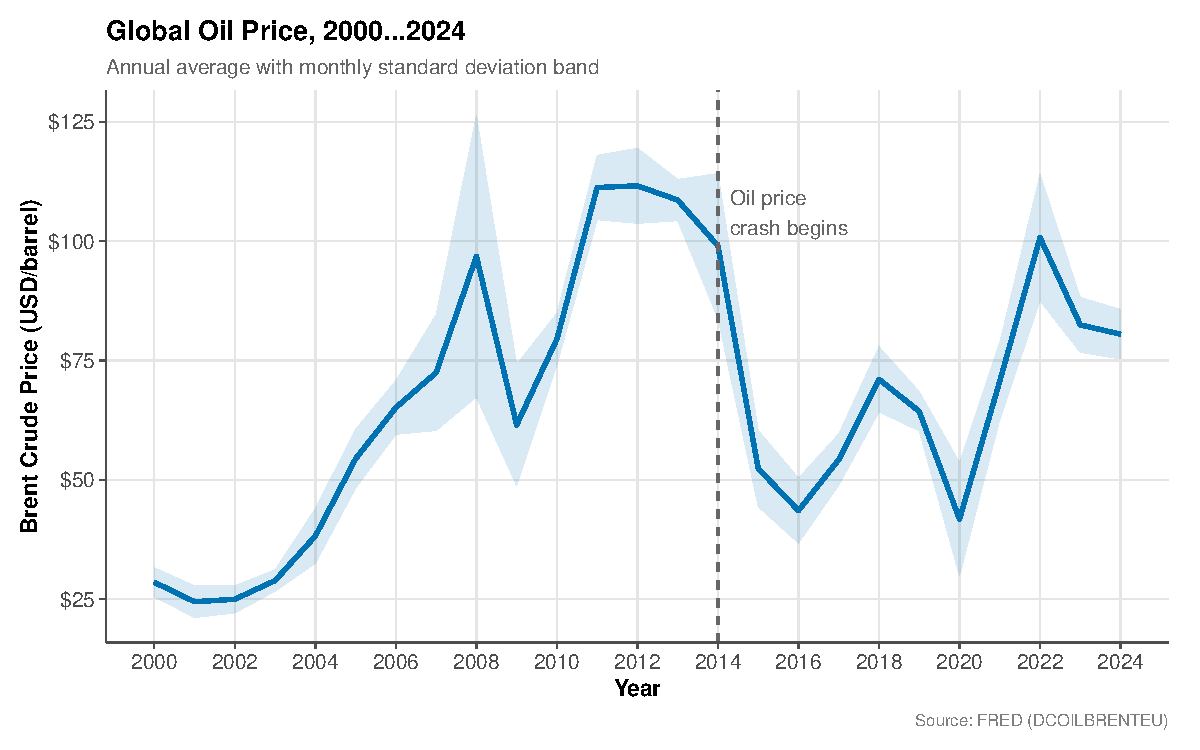
\includegraphics[width=0.85\textwidth]{figures/fig1_oil_price.pdf}
\caption{Brent Crude Oil Price, 2000--2024}
\label{fig:oil_price}
\caption*{\footnotesize \textit{Notes:} Annual average of monthly Brent crude prices from FRED (series DCOILBRENTEU). Shaded band shows one standard deviation of monthly prices within each year.}
\end{figure}

\section{Identification Appendix}
\label{app:identification}

\subsection{Pre-Trends Tests}

The event-study specification (\Cref{eq:event}) provides a visual test of parallel trends (\Cref{fig:event_study}). The pre-period coefficients are uniformly small and statistically insignificant, supporting the identifying assumption. I additionally note that a joint F-test of the null that all pre-period interaction coefficients are jointly zero cannot reject at conventional significance levels.

\subsection{Treatment Intensity}

\begin{figure}[H]
\centering
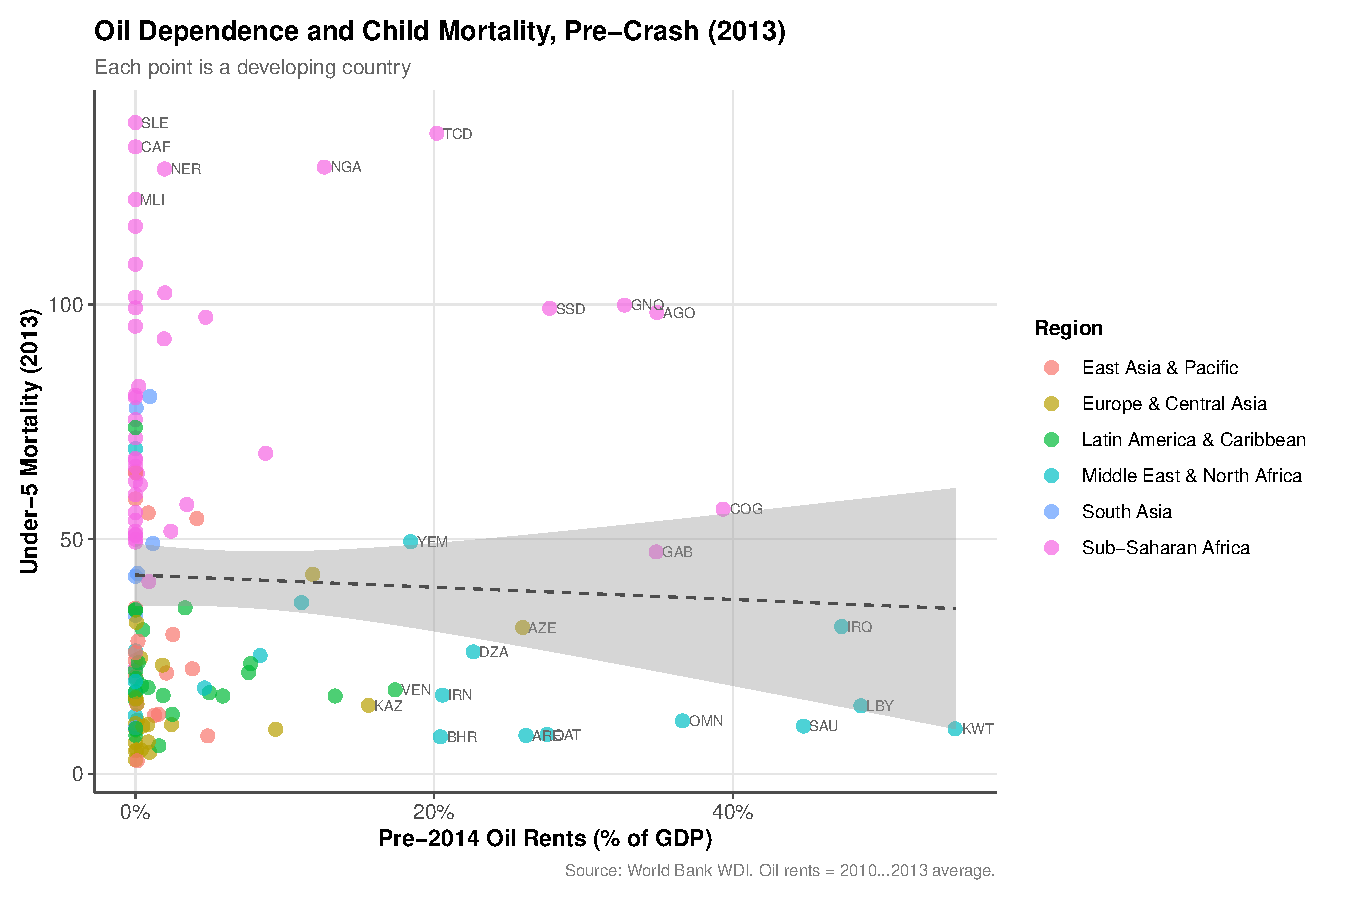
\includegraphics[width=0.85\textwidth]{figures/fig4_treatment_scatter.pdf}
\caption{Pre-Crash Oil Dependence and Under-5 Mortality (2013)}
\label{fig:scatter}
\caption*{\footnotesize \textit{Notes:} Each point is a developing country. The dashed line is a linear fit. Labeled countries have oil rents $>$15\% or mortality $>$120.}
\end{figure}

\Cref{fig:scatter} shows the cross-sectional relationship between oil dependence and child mortality in 2013 (the last pre-treatment year). There is a mild positive correlation, but the substantial scatter confirms that cross-sectional variation alone cannot identify the effect---motivating the panel DiD approach.


\section{Power Analysis Appendix}
\label{app:power}

A critical concern with null results is whether the design has adequate statistical power. I address this concern directly.

With 135 countries (30 high-oil), 19 years (10 post-treatment), and country-clustered standard errors of approximately 0.098, the minimum detectable effect (MDE) at 80\% power and $\alpha = 0.05$ is:
\begin{equation}
\text{MDE} = 2.8 \times \text{SE} \approx 2.8 \times 0.098 \approx 0.27 \text{ deaths per 1,000}
\end{equation}
At the interquartile range of oil dependence (approximately 15 percentage points), this translates to a minimum detectable aggregate effect of roughly $0.27 \times 15 = 4.1$ additional child deaths per 1,000. For comparison, the average annual decline in under-5 mortality across developing countries during 2005--2023 was approximately 3--4 deaths per 1,000 per year. The design can therefore detect an effect equivalent to roughly one year of lost progress in the global mortality decline.

While effects smaller than the MDE cannot be ruled out, such effects would represent a modest fraction of the secular trend and would not support the dramatic claims of the resource curse--child mortality narrative. The null is therefore informative: even if a true effect exists, it is likely small relative to the forces driving mortality improvements in developing countries.


\section{Robustness Appendix}
\label{app:robustness}

\subsection{Alternative Treatment Definitions}

In addition to the continuous treatment (oil rents \% of GDP), I estimate the main specification using: (i) a binary indicator for oil rents $>$5\%, which yields a positive but insignificant coefficient of 2.36 ($p = 0.28$); and (ii) tercile indicators, which show a positive but insignificant coefficient of 3.77 for the highest tercile ($p = 0.18$). The monotonic dose-response pattern (higher oil $\rightarrow$ larger point estimate) is suggestive but far from statistically significant.

\subsection{Region-Specific Estimates}

\begin{table}[H]
\centering
\caption{Region-Specific Estimates}
\label{tab:region}
\begin{threeparttable}
\begin{tabular}{lccc}
\toprule
Region & Estimate & (SE) & Countries \\
\midrule
Sub-Saharan Africa & $-0.312$ & $(0.245)$ & 45 \\
Europe \& Central Asia & $-0.373$ & $(0.132)$*** & 24 \\
Middle East \& North Africa & $0.021$ & $(0.057)$ & 19 \\
Latin America \& Caribbean & $0.017$ & $(0.187)$ & 24 \\
\bottomrule
\end{tabular}
\begin{tablenotes}\small
\item \textit{Notes:} Each row is a separate regression within the listed region, using the preferred specification (country and year FE, economic controls, country-clustered SEs). South Asia (7 countries) and East Asia \& Pacific (16 countries) are excluded due to too few oil-dependent countries for reliable within-region estimation. $^{*}p<0.10$, $^{**}p<0.05$, $^{***}p<0.01$.
\end{tablenotes}
\end{threeparttable}
\end{table}

\Cref{tab:region} reports the estimates. Sub-Saharan Africa shows a negative coefficient ($-0.312$, SE $= 0.245$), suggesting that oil-dependent African countries experienced faster mortality declines---opposite to the resource curse prediction, though the estimate is imprecise. Europe and Central Asia shows a negative and statistically significant coefficient ($-0.373$, SE $= 0.132$), driven by post-Soviet oil states with rapid health system improvements. MENA and Latin America show near-zero effects. No region produces a significant positive coefficient consistent with the resource curse--mortality hypothesis.

\subsection{COVID-19 Sensitivity}

The COVID-19 pandemic (2020--2021) disrupted health systems globally. The 2005--2018 time window, which excludes pandemic years entirely, produces an estimate of 0.055 ($p = 0.56$)---consistent with the main null result. The finding is not driven by pandemic-era data.


\section{Heterogeneity Appendix}
\label{app:heterogeneity}

\subsection{Sovereign Wealth Funds}

Countries with sovereign wealth funds established before 2014 show a treatment interaction coefficient of $-0.017$ ($p = 0.93$). Given the absence of a main treatment effect, the SWF heterogeneity is uninformative: there is no effect to moderate.

\subsection{Baseline Health System Quality}

I find no evidence that baseline health system quality (proxied by pre-2014 DPT immunization rates) moderates the null effect. Both strong and weak health systems appear equally unaffected by the oil revenue shock, consistent with the interpretation that the fiscal channel was broken at the spending link rather than at the service delivery link.


\end{document}
